\documentclass[12pt]{article}
\usepackage{KTUstyle}



\begin{document}
% Titulinis puslapis
\begin{titlepage}

\newcommand{\universitetas}{Kauno technologijos universitetas}
\newcommand{\fakultetas}{Informatikos fakultetas}
\newcommand{\modulioKodas}{Modulio P170B400}
\newcommand{\pavadinimas}{„Algoritmų sudarymas ir analizė“}
\newcommand{\darboTipas}{Laboratorinio darbo ataskaita}
\newcommand{\laboratorinisDarbas}{Ketvirtas laboratorinis darbas}
\newcommand{\autorius}{Vardenis Pavardenis IFF-2/2}
\newcommand{\statusas}{Studentas}
\newcommand{\destytojasOne}{Asist. Pavardenis Vardenis}
\newcommand{\destytojasTwo}{doc. Pavardenis Vardenis}
\newcommand{\destytojai}{Dėstytojai}
\newcommand{\miestas}{Kaunas}
\newcommand{\metai}{2024}

\renewcommand{\headrulewidth}{0pt}

\onehalfspacing
\center

\includegraphics[width=30mm]{KTU logotype_RGB_without text_BLACK} \\ [5mm]
\textbf{\universitetas} \\ [5mm]
\textbf{\fakultetas} \vfill

\textbf{\modulioKodas} \\ [5mm]
\LARGE\textbf{\pavadinimas} \\ [10mm]
\normalsize\textbf{\darboTipas} \\ [5mm]
\textbf{\laboratorinisDarbas} \vfill

\begin{flushright}
\begin{tabular}{l}
\rule{0.9\textwidth}{0.4pt} \\ [0.5cm]
\textbf{\autorius} \\ [5pt]
\textbf{\statusas} \\ [15pt]
\textbf{\destytojasOne} \\ [5pt]
\textbf{\destytojasTwo} \\ [5pt]
\textbf{\destytojai} \\ [1.5cm]
\rule{0.9\textwidth}{0.4pt}
\end{tabular}
\end{flushright}

\vfill
\center
\textbf{\miestas} \\
\textbf{\metai}

\end{titlepage}
		

% Turinys
\tableofcontents

\newpage


\section{Dokumento elementai}

\subsection{Sąrašai}

\paragraph{Pavyzdyje bus pateikta:}	
\begin{enumerate}
	\item Formulės (\ref{formules} skyrius):
	\begin{enumerate}
		\item vienos eilutės (\ref{vienos} skyrius),
		\item kelių eilučių  (\ref{keliu} skyrius).
	\end{enumerate}
	\item Lentelės (\ref{lenteles} skyrius).
	\item Paveikslai (\ref{paveikslai} skyrius).
	\item Literatūros sąrašas (\pageref{literatura} puslapis).
\end{enumerate}

\paragraph{LaTeX, dokumentacijas galite rasti:}
\begin{itemize}
	\item http://latex-project.org/guides/
	\item http://www.maths.tcd.ie/~dwilkins/LaTeXPrimer/
	\item https://www.google.com
\end{itemize}

\subsection{Formulės} \label{formules}
\eqref{eq:2} pateikta vienos eilutės formulė, \eqref{eq:1} -- dviejų eilučių formulė.

\subsubsection{Vienos eilutės formulė} \label{vienos}
\begin{equation}
	f = \bar{x}_{1}\bar{x}_{2}\bar{x}_{3}\bar{x}_{4}\bar{x}_{5}\bar{x}_{6}\cup x_{1}\bar{x}_{2} x_{3} x_{4} x_{5}\bar{x}_{6}. \label{eq:2}
\end{equation}

\subsubsection{Kelių eilučių formulė} \label{keliu}
    \input{neminimizuota_funkcija.txt}  
 

 
\subsection{Lentelės} \label{lenteles}

\begin{table}[!htbp]
\caption{Funkcijos teisingumo lentelė.}
	\centering
	\begin{tabular}{|cc|c|}
		\hline
		$x_1$ & $x_2$ & $y$ \\
		\hline
		0 & 0 & 1 \\
		0 & 1 & 0 \\
		1 & 0 & 0 \\
		1 & 1 & 1 \\
		\hline
	\end{tabular}
\end{table}


\subsection{Paveikslai} \label{paveikslai}

\ref{fig:11} pav. pavaizduotas pirmasis namas, \ref{fig:12} pav. -- antrasis namas. \ref{fig:2} pav. pirmasis namas pavaizduotas didesniu formatu. 

\begin{figure}[!htbp] 
\centering
\subfloat[Pirmas namas]{\label{fig:11}%
  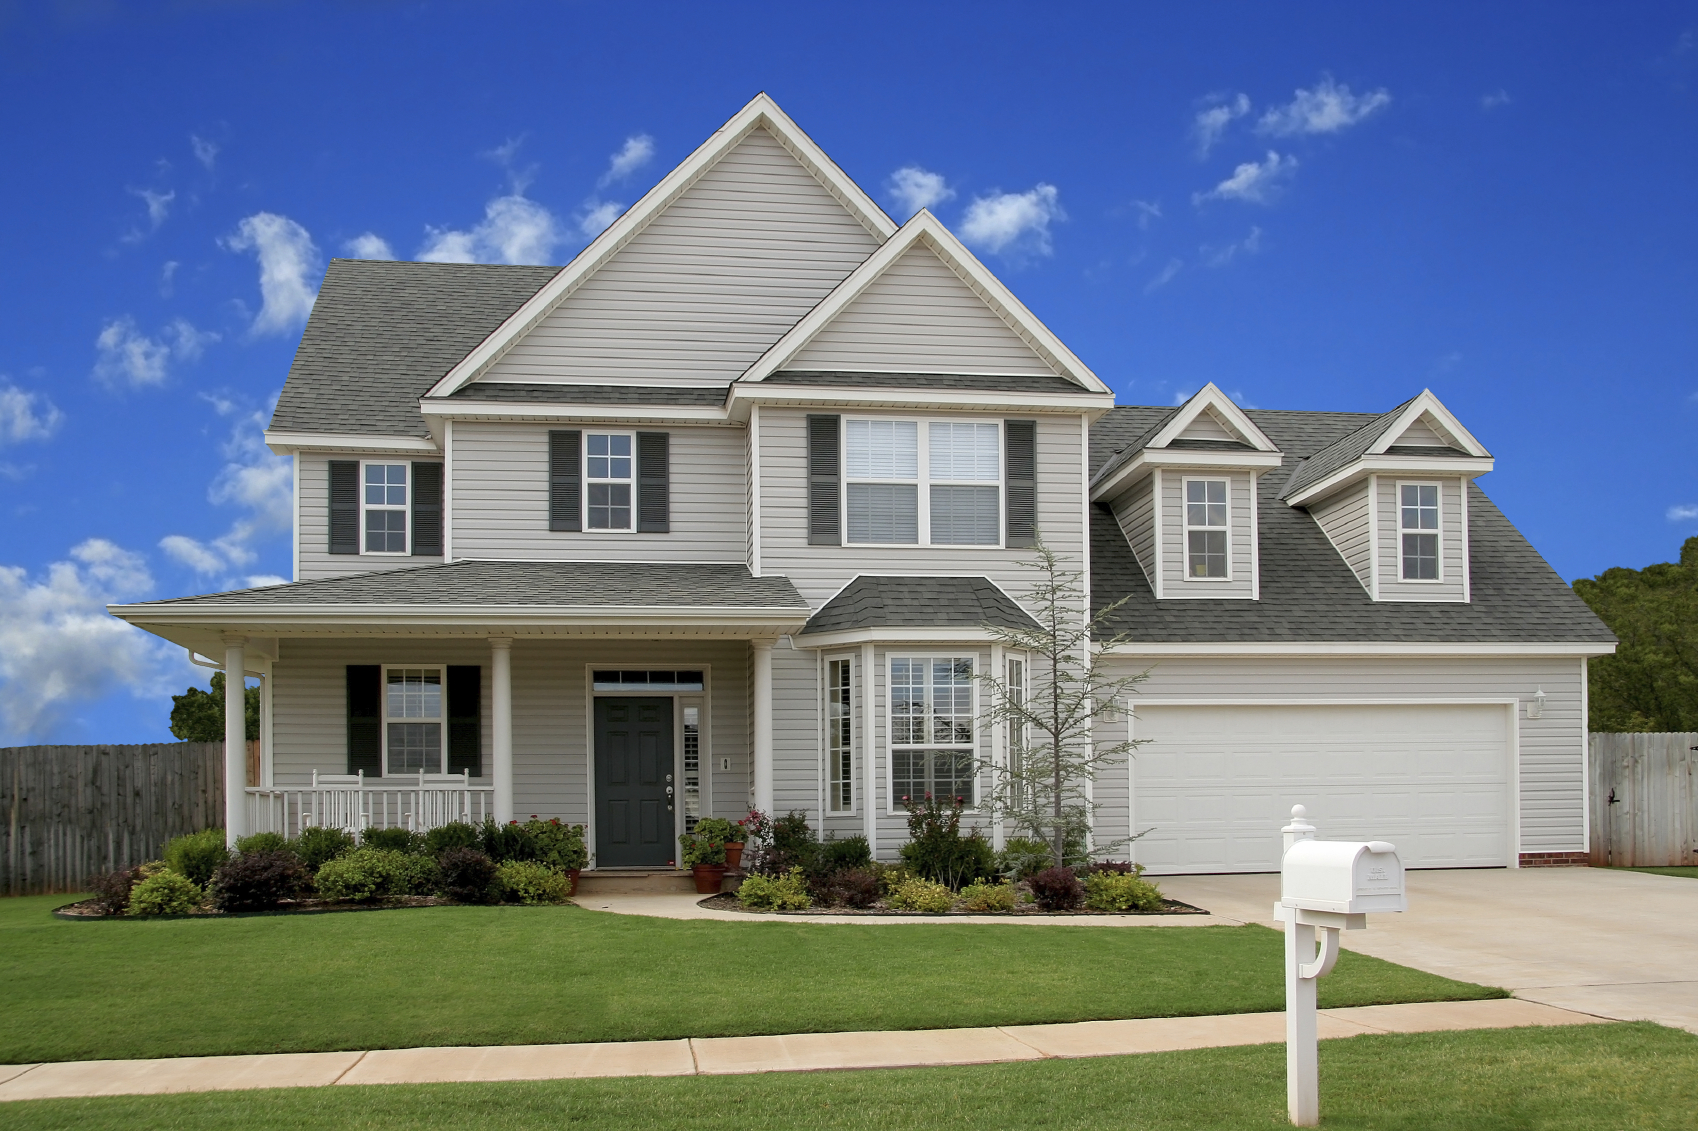
\includegraphics[height=5cm]{house1}}\ %
\subfloat[Antras namas]{\label{fig:12}%
  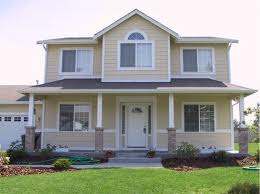
\includegraphics[height=5cm]{house2}}
\caption{Pirmas ir antras namai.}
\label{fig:1} 
\end{figure} 

\begin{figure}[!htbp]
\centering
	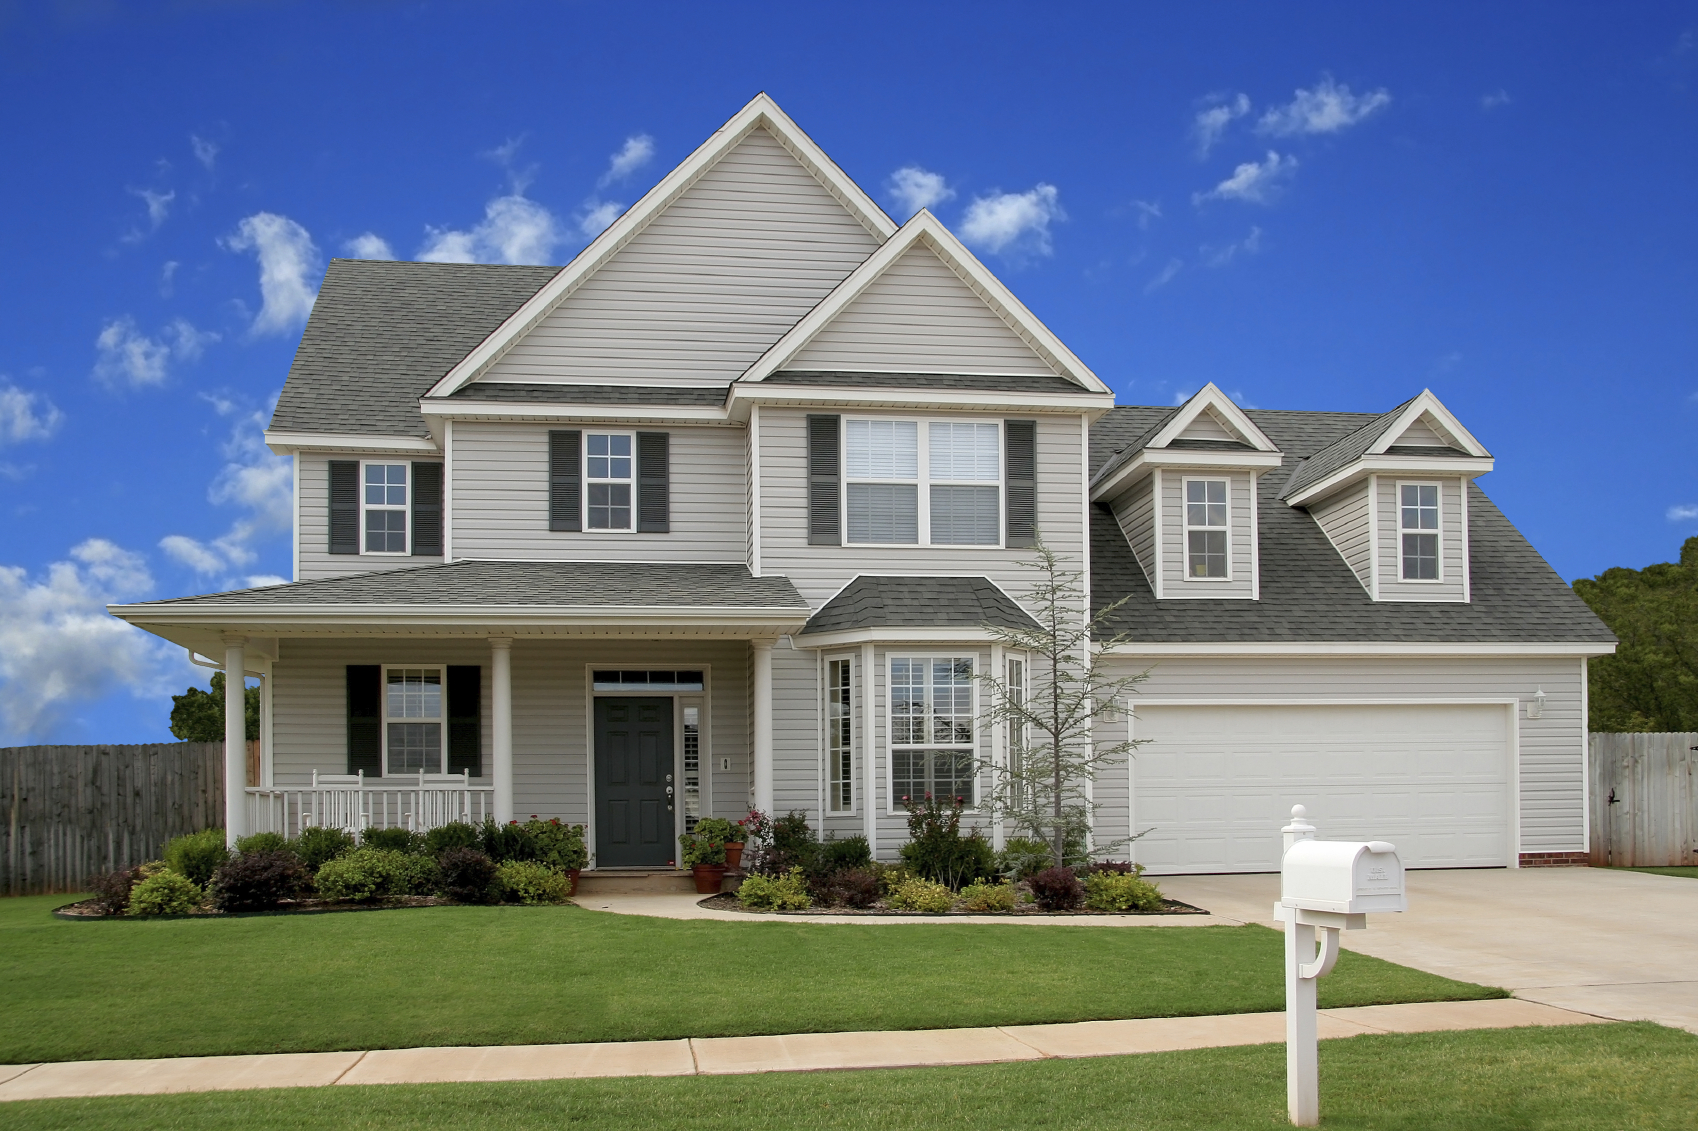
\includegraphics[height=8cm]{house1}
	\caption{Didelis pirmas namas.}
	\label{fig:2}
\end{figure}

\ref{fig:2} pav. namą galima rasti \cite{namas} šaltinyje.

\newpage
% Literaturos sarasas
\newpage

\bibliographystyle{plain}  
\begin{thebibliography}{99}

%\phantomsection
\addcontentsline{toc}{section}{Literatūra}\label{literatura}


\bibitem{meng}
Meng X. Implantable Wireless Devices for the Monitoring of Intracranial 
Pressure // X. Meng, U. Kawoos, S. M. Huang, M. R. Tofighi // IEEE 16th International Symposium. -- 2012.


\bibitem{north}
North B. Intracranial pressure monitoring //P. Reilly, R. Bullock. Head Injury; Chapman \& Hall, London, 1997.

\bibitem{popovic}
Popovic D. Noninvasive Monitoring of Intracranial Pressure / D. Popovic, M. Khoo, S. Lee // Recent Patents on Biomedical Engineering. -- 2009, 2, p. 165-179.

\bibitem{namas} 
http://streetinfo.com/6-tips-hosting-great-open-house/

\end{thebibliography}

\end{document}

